\chapter{轨道交通联锁软件可信量化评估模型}
\label{ch3}

\begin{kaishu}
文献\cite{Hasselbring2006Toward}认为不同属性之间可能存在本质上或外在的联系,将属性分离出来研究不足以体现实际软件系统设计问题的复杂性。目前涉及属性之间的关系模型研究大多是基于经验从定性的角度出发,对于可信属性之间关系的量化没有较为系统的研究\cite{张卫祥2015软件可信性定量评估}。
根据轨道交通联锁软件的项目需求,
% 主要立足于四个可信属性,分别为功能性、可靠性、安全性和可维护性。
本章首先建立轨道交通联锁软件的可信评估指标体系;然后构建轨道交通联锁软件的结构方程模型,得出度量元,子属性,属性的权重;
最后结合软件可信度量模型与量化分级方法计算轨道交通联锁软件的可信值并进行可信等级的划分。
\end{kaishu}

\section{轨道交通联锁软件可信评估指标体系}
\subsection{评估指标体系建立的原则}
软件可信评估所涉及的可信属性是多维的,动态的,评估指标比较复杂,涉及的范围比较广泛。
正是由于软件可信评估体系内部变量选取的复杂与困难,根据相关理论研究,
%由于软件可信评估指标体系中可信属性的复杂性特点,根据复杂系统理论与管理决策理论,
列出了可信评估指标体系建立依据的六个原则,
分别是目标性、可比性、科学性、独立性、系统性和实用性\cite{戴君2015基于结构方程模型的可持续供应链绩效评价研究}。

\subsection{可信评估指标体系的建立}
本文是基于轨道交通联锁软件全生命周期进行可信评估,最后综合每个阶段的可信值计算软件整体的可信值。在实验室团队研究成果的基础上,对需求、设计、编码和测试四个阶段建立可信评估指标体系。
为了保持前后阶段的一致性,属性在每个阶段一样,同时由于每个阶段针对属性具体做的事情的不同,各个阶段设计的度量元有所不同。
开发一个软件首先要做的事情就是进行需求分析,确定这个软件到底是要做什么,是后续工作的基础\cite{汪莹2012浅谈软件需求分析}。
% 需求阶段是软件开发的第一步,给后续阶段的工作提供指导作用,对于软件需要“做什么”进行了详细的分析。
本文主要介绍需求阶段可信评估指标体系的建立与结构方程模型的构建。评估目标是每个阶段可信性,一级评估指标对应属性,二级评估指标对应度量元。

在需求阶段,对功能性来说,功能定义充分程度、功能定义适配程度、功能定义正确程度、接口关系、协议、数据定义完整程度、接口可扩展程度是其二级评估指标,分别用X1至X5表示。可靠性通过成熟性要求定义充分程度、需求稳定性程度、错误处理规则识别程度、失效种类和失效后处理措施明确程度来反映,分别用X6至X9表示。\cite{郭婉琴2014一种机载软件安全性需求获取方法}安全性的二级评估指标包括通用和特定安全需求定义充分程度、软件安全性功能需求充分且需求标识定义完整程度、防危性要求定义充分程度、危险日志明确程度,分别用X10至X13表示。可维护性二级评估指标为双向追踪关系明确程度、问题分析定位能力、合格性审查要求明确程度、修改可再确认能力,分别用X14至X17表示。为了让用户深入了解软件产品的可信性,从用户角度出发建立一套评估指标也是必要的。对于软件可信性这个评估目标而言,将用户对该软件的使用反馈作为其评估指标,包含软件功能满意程度、软件运行稳定程度,软件用户交互友好程度,分别用Y1、Y2和Y3表示。

在建立评估指标体系时,首先用四个基本可信属性对抽象的软件可信性进行分解,再对四个属性进一步分解成可以直接获得观测数据的具体指标,相关从事人员可以依据具体指标的表现追根溯源,提出改进方案。需求阶段可信评估指标体系如表\ref{tab-3-1}所示:
\begin{table}[htbp]
	\centering
	\caption{需求阶段可信评估指标体系}\label{tab-3-1}
	\begin{tabular}[htbp]{|l|l|l|c|}
		    \hline
			评估目标 & 一级评估指标 & 二级评估指标 & 符号\\
			\hline
			\multirow{17}*{\tabincell{l}{需求阶段可信性}} &
			\multirow{5}*{\tabincell{l}{功能性}}&功能定义充分程度 & X1\\ \cline{3-4} 
			& &功能定义适配程度 & X2\\ \cline{3-4} 
			& &功能定义正确程度 & X3\\ \cline{3-4} 
			& &\tabincell{l}{接口关系、协议、数据定义完整程度} & X4\\ \cline{3-4}
			& &接口可扩展程度 & X5\\
			\cline{2-4} &
			\multirow{4}*{\tabincell{l}{可靠性}} &成熟性要求定义充分程度 & X6\\ \cline{3-4}
			& &需求稳定性程度 & X7\\ \cline{3-4}
			& &错误处理规则识别程度 & X8\\ \cline{3-4}
			& &\tabincell{l}{失效种类和失效后处理措施明确程度} & X9\\ \cline{3-4}
			\cline{2-4} &
			\multirow{4}*{\tabincell{l}{安全性}} & \tabincell{l}{通用和特定安全需求定义充分程度} & X10\\ \cline{3-4}
			& &\tabincell{l}{软件安全性功能需求充分且需求标识\\定义完整程度} & X11\\ \cline{3-4}
			& &防危性要求定义充分程度 & X12\\ \cline{3-4}
			& &危险日志明确程度 & X13\\ \cline{3-4}
			\cline{2-4} &
			\multirow{4}*{\tabincell{l}{可维护性}} &双向追踪关系明确程度 & X14\\ \cline{3-4}
			& &问题分析定位能力 & X15\\ \cline{3-4}
			& &合格性审查要求明确程度 & X16\\ \cline{3-4}
			& &修改可再确认能力 & X17\\
			\hline
	\end{tabular}
\end{table}


本文用于需求阶段可信性评估的一级评估指标属性有功能性、可靠性、安全性、可维护性,假设17个二级评估指标之间没有重叠,保持相互独立。在实际开发的软件系统中,功能性、可靠性、安全性、可维护性是相互作用的。
例如,如果对于安全性要求和功能性要求之间的冲突没有进行妥善处理,会对系统的可信性产生影响,可见安全性与功能性是存在内在关联的关系的;
要想在地铁运行期间保证其安全性和功能性的目标,必须要实现可维护性和可靠性的要求,并且对于正在进行或者是周期很长的维护和运行活动以及运行环境都要严格控制。
% 例如,从对安全性要求和功能性要求之间的冲突管理不善就会妨碍获得系统可信性的角度来看,安全性和功能性是内在关联的。只有满足可靠性和可维护性的所有要求,并控制正在进行的或长期的维护和运行活动以及运行环境,才能达到运行期间的安全性和功能性目标\cite{EN50126}。

\section{轨道交通联锁软件可信评估结构方程模型}
\subsection{模型构建}
根据上文建立的联锁软件可信评估指标体系,构建测量模型。由于受到四个属性的影响,软件可信性不可直接观测,作为内生潜变量;四个属性概念也比较抽象,还需进一步分解,则可作为外生潜变量;从用户角度考虑的三个指标可作为内生观测变量;因此,测量模型包括功能性、可靠性、安全性和可维护性四个外生潜变量,还有潜变量的17个观测指标;内部观测指标则以软件功能满意程度、软件运行稳定程度,软件用户交互友好程度表示;e1至e21为误差项。
使用AMOS25.0绘制路径关系图,建立的轨道交通联锁软件需求阶段的结构方程模型如图\ref{fig:3_01}所示:
\begin{figure}[htb]
	\centering
	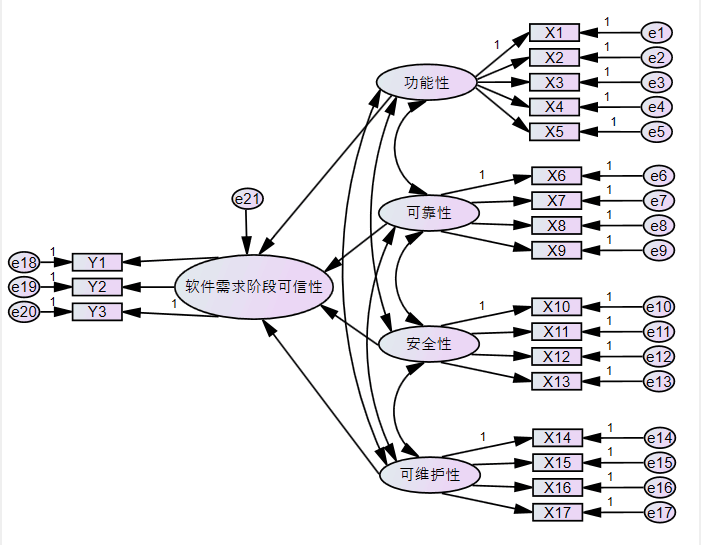
\includegraphics[width=13cm]{fig/3_1.png}
	\caption{轨道交通联锁软件需求阶段的结构方程模型}
	\label{fig:3_01}
\end{figure}

\subsection{模型设定}
初步假设不同潜变量的观测变量之间没有相关关系,根据假设使用Amos绘制的路径图如图所示。
\begin{figure}[htb]
	\centering
	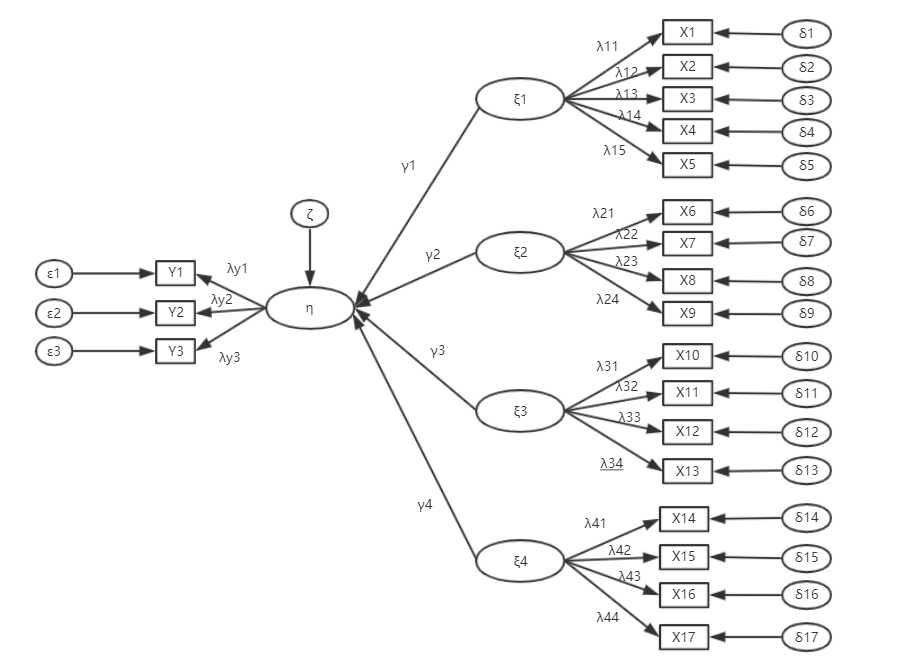
\includegraphics[width=13cm]{fig/3_02.png}
	\caption{可信评估结构方程模型路径图}
	\label{fig:3_02}
\end{figure}

根据上图,对于测量模型来说,外生潜变量有4个,因此$\xi$为4*1阶矩阵;内生潜变量只有1个,所以$\eta$为1阶矩阵。对于结构模型来说,$\Gamma$为外因潜变量对内因潜变量的影响,是一个4*1阶矩阵。$\zeta$为残差项,是1阶矩阵\cite{赵怡晴2016产品质量风险监控绩效评估的结构方程模型}。

$\gamma_1、\gamma_2、\gamma_3、\gamma_4$表示外生潜变量对内生潜变量路径系数,分别是$\xi_1、\xi_2、\xi_3、\xi_4$对内生潜变量$\eta$分别表示的影响程度。

$X_1-X_{17}$是$\xi$的观测变量,$Y_1-Y_3$是$\eta$的观测变量。$\lambda_{ij}$是因素负荷量,反映的是观测变量对外生潜变量的反映程度。因此,根据测量方程式\ref{formula:x}和\ref{formula:y},得出的轨道交通联锁软件可信评估的测量模型如下:
\begin{align}
    x=\Lambda_x\xi+\delta \\
    y=\Lambda_y\eta+\varepsilon\\
    \eta=\Gamma\xi+\zeta 
\end{align}
也可采用矩阵来表示上述模型之间的关系
\begin{gather}
\begin{pmatrix}
X_1\\
X_2\\
\cdots \\
X_{16}\\
X_{17}
\end{pmatrix}=
\begin{pmatrix}
\lambda_{11} & 0 & 0 & 0 \\
\cdots & \cdots & \cdots & \cdots \\
\lambda_{15} & 0 & 0 & 0 \\
0 & \lambda_{21} & 0 & 0 \\
\cdots & \cdots & \cdots & \cdots \\
0 & \lambda_{24} & 0 & 0 \\
0 & 0 & \lambda_{31} & 0 \\
\cdots & \cdots & \cdots & \cdots \\
0 & 0 & \lambda_{34} & 0 \\
0 & 0 & 0 & \lambda_{41} \\
\cdots & \cdots & \cdots & \cdots \\
0 & 0 & 0 & \lambda_{44} 
\end{pmatrix}
\begin{pmatrix}
\xi_1\\
\xi_2\\
\xi_3 \\
\xi_4
\end{pmatrix}
+
\begin{pmatrix}
\delta_1\\
\delta_2\\
\cdots \\
\delta_{16}\\
\delta_{17}
\end{pmatrix}
\end{gather}


\begin{gather}
\begin{pmatrix}
Y_1\\
Y_2\\
Y_3
\end{pmatrix}
=
\begin{pmatrix}
\lambda_{y11}\\
\lambda_{y21}\\
\lambda_{y31}
\end{pmatrix}
\begin{pmatrix}
\eta
\end{pmatrix}
+
\begin{pmatrix}
\epsilon_1\\
\epsilon_2\\
\epsilon_3
\end{pmatrix}
\end{gather}

\begin{gather}
\begin{pmatrix}
\eta
\end{pmatrix}
=
\begin{pmatrix}
\gamma_{11} & \gamma_{12} & \gamma_{13} & \gamma_{14}
\end{pmatrix}
\begin{pmatrix}
\xi_1\\
\xi_2\\
\xi_3 \\
\xi_4
\end{pmatrix}
+
\begin{pmatrix}
\zeta
\end{pmatrix}
\end{gather}




\subsection{模型检验与拟合}

(1)信度检验

信度是指在对同一对象使用相同的手段反复测量时所得结果的一致性程度\cite{张运新2017某校学生对校园文体活动主观感受的调查问卷信度分析}。
% 信度是指采用同样的方法对同一对象重复测量时所得结果的一致性程度\cite{何耀2017公众低碳出行行为决策模型的研究}。
本文对信度检验使用在线SPSS工具,检验标准通常参考Cronbach’s Alpha系数。一般$\alpha$系数的值在0和1之间,
0.6为下界,小于等于0.6则不足以相信内部的一致性,如果在0.7与0.8之间那么可以接受,
0.8-0.9说明量表信度非常好\cite{Cronbach’sAlpha}。

(2)效度检验

效度指测量对象能否被测量手段或者工具准确测出的程度\cite{赵学金2009基于结构方程的知识型服务质量的评价方法}。
% 效度指测量工具或手段能够准确测出所需测量的事物的程度\cite{赵学金2009基于结构方程的知识型服务质量的评价方法}。
本文采用AMOS25.0进行效度检验。
效度一般分为三类,包括内容效度、准则效度和结构效度。
内容效度过多依赖于主观判断,对于准则效度来说,很难确定一个良好的标准。因此本文针对结构效度进行检验,求出潜变量的平均方差抽取量(AVE),
AVE值的大小若是在0.5以上,表示观测变量可以有效反映其潜变量。

(3)模型拟合

模型拟合是判断所构造的联锁软件可信评估结构方程模型的适配度指标是否达到适配标准。根据文献\cite{乔红丽2017移动图书馆用户体验的结构方程模型分析}所提出的适配统计量,本文选取以下几个常用的适配度指标:
\begin{itemize}
    % \item 卡方值:卡方值越小表示假设的模型路径图与实际情况越适配。
    \item 卡方值与自由度比:若卡房自由度比小于1.0,表示模型过度适配;若其值大于2.0或3.0(较宽松的规定值是5.0)表示假设的模型无法反应真实数据,即需要对模型进行改进,提高模型契合度。
    \item 渐进残差均方和平方根(RMESA):这个值越小,越能说明模型的适配度好。通常情况,值在0.08-0.10之间模型尚可,具有普通适配度;0.05-0.08之间表示模型适配合理;若其小于0.05表示模型的适配度非常好。
    \item 非规范化拟合指数(TLI):数值大于0.09,则认为模型契合度良好。
    \item 比较适配指数(CFI):数值大于0.09,则认为模型契合度良好。
    \item 增值适配指数(IFI):数值大于0.09,则认为模型契合度良好。
\end{itemize}
最终本文确定模型适配度的指标检标准验如表\ref{tab-3-2}所示:
\begin{table}[!ht]
	\centering
	\renewcommand\arraystretch{1.3}
	\caption{模型适配度指标检验}
	\begin{tabular}{|l|c|c|c|c|c|c|c|}
% 	{|p{2cm}<{\centering}|p{1.6cm}<{\centering}|p{1.8cm}<{\centering}|p{1.8cm}<{\centering}|p{1.6cm}<{\centering}|p{2.2cm}<{\centering}|p{2.2cm}<{\centering}|}%几列就有几个c
		\hline
		\textbf{拟合标准} & \textbf{CMIN/DF} & \textbf{RFI} & \textbf{IFI} & \textbf{TLI} & \textbf{CFI} & \textbf{RMSEA} \\
		\hline
		参照指标结果 & 大于0.9 & 大于0.9 & 大于0.9 & 大于0.9 & 大于0.9 & 小于0.08 \\
		\hline
	\end{tabular}
	\label{tab-3-2}
\end{table}

\section{示例说明}
由于数据收集是一个漫长的过程,本节针对需求阶段所用到的数据来自第三方的问卷调查,发放给参与过软件开发过程相关的工作人员填写,回收了有效问卷170份。为了更具有区分度,问卷打分参考Likert量表 采用10分制,"非常同意"、"同意"、"不一定"、"不同意"、"非常不同意"五种分别记为10、8、6、4、2,奇数表示的认可程度评价介于其前后两个数字之间。

对收集的数据进行信度分析的结果如表2所示,每个因子的信度都大于0.8,结果表明量表信度非常好。
本文样本数据的信度检验表如\ref{tab-3-3}:
\begin{table}[!ht]
	\centering
	\renewcommand\arraystretch{1.3}
	\caption{信度检验表}
	\begin{tabular}{|c|c|}
% 	{|p{2cm}<{\centering}|p{1.6cm}<{\centering}|p{1.8cm}<{\centering}|p{1.8cm}<{\centering}|p{1.6cm}<{\centering}|p{2.2cm}<{\centering}|p{2.2cm}<{\centering}|}%几列就有几个c
		\hline
		\textbf{因子} & \textbf{Cronbach’s Alpha系数} \\
		\hline
		功能性 & 0.865  \\
		\hline
		可靠性 & 0.896\\
		\hline
		安全性 &  0.882 \\
		\hline
		可维护性  & 0.906 \\
		\hline
		软件可信性 & 0.864 \\
		\hline
	\end{tabular}
	\label{tab-3-3}
\end{table}

然后将数据文件输入到Amos 25.0,轨道交通连锁软件可信评估结构方程模型的标准化之后的结果如下图。
\begin{figure}[htb]
	\centering
	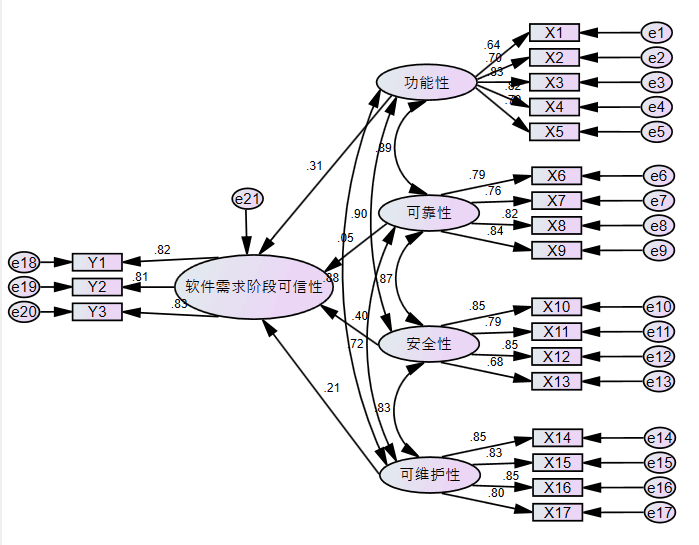
\includegraphics[width=13cm]{fig/3_3.png}
	\caption{轨道交通联锁软件需求阶段的结构方程模型标准化结果}
	\label{fig:3_03}
\end{figure}

样本数据效度分析结果如表\ref{tab-3-4}所示,所有指标因素负荷量的值均在0.5到0.95之间。功能性、可靠性、安全性和可维护性的平均方差抽取量AVE的值均大于0.5,表明量表具有很高的结构效度。
\begin{table}[H]
	\centering
	\caption{需求阶段可信评估效度检验}
	\label{tab-3-4}
	\begin{tabular}[H]{|l|l|l|c|}
		    \hline
			一级评估指标 & 二级评估指标 & 因素负荷量 & AVE(平均方差抽取量)\\
			\hline
			
			\multirow{5}*{\tabincell{l}{功能性}}&功能定义充分程度 & 0.64& \multirow{5}*{0.56}\\ \cline{2-3} 
			&功能定义适配程度 & 0.70& \\ \cline{2-3} 
			&功能定义正确程度 & 0.83&\\ \cline{2-3} 
			&\tabincell{l}{接口关系、协议、数据定\\义完整程度} &0.82 &\\ \cline{2-3}
			&接口可扩展程度 & 0.76&\\
			\hline
			\multirow{4}*{\tabincell{l}{可靠性}} &成熟性要求定义充分程度 & 0.79 &\multirow{4}*{0.64}\\ \cline{2-3}
			&需求稳定性程度 & 0.76&\\ \cline{2-3}
			&错误处理规则识别程度 & 0.82 &\\ \cline{2-3}
			&\tabincell{l}{失效种类和失效后处理措\\施明确程度} & 0.84 &\\ 
			\hline
			\multirow{4}*{\tabincell{l}{安全性}} & \tabincell{l}{通用和特定安全需求定\\义充分程度} & 0.85 &\multirow{4}*{0.63}\\ \cline{2-3}
			&\tabincell{l}{软件安全性功能需求充分\\且需求标识定义完整程度} & 0.79&\\ \cline{2-3}
			&防危性要求定义充分程度 & 0.85&\\ \cline{2-3}
			&危险日志明确程度 & 0.68 &\\ 
			\hline
			\multirow{4}*{\tabincell{l}{可维护性}} &双向追踪关系明确程度 & 0.85 & \multirow{4}*{0.69}\\ \cline{2-3}
			&问题分析定位能力 & 0.83&\\ \cline{2-3}
			&合格性审查要求明确程度 & 0.85 &\\ \cline{2-3}
			&修改可再确认能力 & 0.80&\\
			\hline
	\end{tabular}
\end{table}

表\ref{tab-3-5}为模型拟合的适配度指标结果,从表中可以得出模型拟合效果从整体而言,是可以接受的。

%\begin{figure}[htb]
%	\centering
%	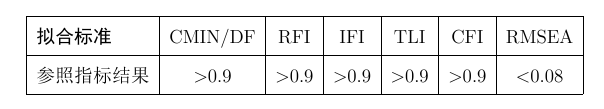
\includegraphics[width=13cm]{fig/3_04.png}
%	\caption{示例适配度指标检验结果}
%	\label{fig:3_04}
%\end{figure}

\begin{table}[!ht]
	\centering
	\renewcommand\arraystretch{1.3}
	\caption{示例适配度指标检验结果}
	\begin{tabular}{|l|c|c|c|c|c|c|c|}
		\hline
		\textbf{统计检验量} &  \textbf{CMIN/DF} & \textbf{RFI} & \textbf{IFI} & \textbf{TLI} & \textbf{CFI} & \textbf{RMSEA} \\
		\hline
		适配标准  & <3 & >0.9 & >0.9 & >0.9 & >0.9 & <0.08 \\
		\hline
		适配结果 & 2.074 & 0.842 & 0.934 & 0.912 & 0.933 & 0.079   \\
		\hline
	\end{tabular}
	\label{tab-3-5}
\end{table}

接下来对轨道交通联锁软件需求阶段可信性进行评估,具体步骤:首先得到每一个观测变量的分值,然后进行观测变量的因素负荷量归一化分别计算对应度量元的权重和子属性的权重,最后根据分值和权重结合公式\ref{formula:zishuxingkexinzhi}、\ref{formula:shuxingkexinzhi}和\ref{formula:jieduankexinzhi}自下而上计算需求阶段可信值,如表\ref{tab-3-6}所示:
\begin{table}[htbp]
	\centering
	\caption{需求阶段可信评估}
	\label{tab-3-6}
	\begin{tabular}[htbp]{|c|c|c|c|c|c|c|c|}
		    \hline
			\tabincell{l}{总目标} & \tabincell{l}{外生潜变\\量(属性)} & 权重 & 子属性 & 权重 & \tabincell{l}{观测变量\\(度量元)}& 权重 & 分值  \\
			\hline
			\multirow{17}*{\tabincell{c}{阶段\\可信值\\7.12}} &
			\multirow{5}*{\tabincell{c}{功能性\\7.10}} & \multirow{2}*{\tabincell{l}{0.32}} &  \multirow{2}*{\tabincell{c}{适合性\\7.48}} & \multirow{2}*{\tabincell{l}{0.36}} &  X1 & 0.17 & 7.32\\ \cline{6-8} 
			& & & & & X2 & 0.19 & 7.63\\ \cline{4-8} 
			& & &  \tabincell{c}{准确性\\7.83}  & 0.22 & X3 & 0.22 & 7.83\\ \cline{4-8} 
			& & &  \multirow{2}*{\tabincell{c}{互操作性\\6.44}} & \multirow{2}*{\tabincell{l}{0.42}} & X4 & 0.22 & 6.73\\ \cline{6-8}
			& & &  & & X5 & 0.20 & 6.12\\
			\cline{2-8}
			& \multirow{4}*{\tabincell{c}{可靠性\\6.84}} & \multirow{2}*{\tabincell{l}{0.05}} &  \multirow{2}*{\tabincell{c}{成熟性\\6.79}} & \multirow{2}*{\tabincell{l}{0.48}} &  X6 & 0.24 & 6.81\\ \cline{6-8} 
			& &  & & & X7 & 0.24 & 6.76\\ \cline{4-8} 
			& & &  \multirow{2}*{\tabincell{c}{容错性\\6.88}} & \multirow{2}*{\tabincell{l}{0.52}} &  X8 & 0.26 & 7\\ \cline{6-8}
			& & & & & X9 & 0.26 & 6.75\\
			\cline{2-8} 
			& \multirow{4}*{\tabincell{c}{安全性\\7.34}} & \multirow{2}*{\tabincell{l}{0.41}} &  \multirow{2}*{\tabincell{c}{安全完善性\\7.25}} & \multirow{2}*{\tabincell{l}{0.52}} & X10 & 0.27 & 7.12\\ \cline{6-8} 
			& &  & & & X11 & 0.25 & 7.39 \\ \cline{4-8} 
			& & &  \multirow{2}*{\tabincell{c}{防危性\\7.44}} & \multirow{2}*{\tabincell{l}{0.48}} &  X12 & 0.27 & 7.26\\ \cline{6-8}
			& & & & & X13 & 0.21 & 7.68\\
			\cline{2-8} 
			& \multirow{4}*{\tabincell{c}{可维护性\\6.81}} & \multirow{2}*{\tabincell{l}{0.22}} &  \multirow{2}*{\tabincell{c}{易分析性\\6.98}} & \multirow{2}*{\tabincell{l}{0.5}} &  X14 & 0.26 & 7.25 \\ \cline{6-8} 
			& &  & & & X15 & 0.24 & 6.69\\ \cline{4-8} 
			& & &  \multirow{2}*{\tabincell{c}{易测试性\\6.64}} & \multirow{2}*{\tabincell{l}{0.5}} &  X16 & 0.26 & 6.54\\ \cline{6-8}
			& &  & & & X17 & 0.24 & 6.74\\
			\hline
	\end{tabular}
\end{table}

设计、编码和测试三个阶段的可信评估过程类似于需求阶段。假设其他三个阶段的数据和需求阶段是一样的,每个阶段同等重要所以占的权重相等,均为0.25,根据公式\ref{formula:ruanjiankexinzhi},得出软件整体的可信值为$7.12^{0.25}*7.12^{0.25}*7.12^{0.25}*7.12^{0.25}=7.12$,对应软件可信量化分级模型表,第二列软件的可信值大于7.0,没有可信值低于7.0的阶段,但每个阶段都有两个属性的可信值介于4.5和7之间,不能满足\uppercase\expandafter{\romannumeral3}级条件,所以软件的可信等级为\uppercase\expandafter{\romannumeral4}级。


\section{本章小结}
本章介绍了轨道交通联锁软件的可信量化评估模型。该模型首先包括可信评估体系的建立,然后在评估体系的基础上构建结构方程模型,最后结合度量模型与可信量化分级模型表得出软件可信值与等级。在章末阐述了一个示例进行具体说明。
